% !TEX root = main.tex
    \hspace{-22mm}
    \begin{subfigure}[htp]{0.4\textwidth}
\begin{tikzpicture}[scale=1.7]
\node[scale=2.8] at (-0.4,0){$\rho$};
\node[scale=4.7] at (4.5,1.15){% !TEX root = main.tex

\begin{tikzpicture}

\coordinate (A) at (-1.20,-0.055);
\coordinate (B) at (-1.21,-0.245);
\coordinate (C) at (-0.79,-0.245);
\coordinate (D) at (-0.80,-0.055);
% \draw (A)--(B) -- (C) -- (D) -- cycle;
\draw [fill=red!60, draw=none, color=red!60,  rounded corners=0.14mm] (A) -- (B) -- (C) -- (D) -- cycle;
\draw [red!80, line width=0.1, line cap=round] (-1.15, 0.0) to [out=260,in=80] (-1.2, -0.242);
\draw [red!80, line width=0.1, line cap=round] (-1.15+0.04, 0.05) to [out=260,in=80] (-1.2+0.05, -0.242);
\draw [red!80, line width=0.1, line cap=round] (-1.15+0.08, 0.05) to [out=262.5,in=82.5] (-1.2+0.1, -0.242);
\draw [red!80, line width=0.1, line cap=round] (-1.15+0.12, 0.05) to [out=265,in=85] (-1.2+0.15, -0.242);
\draw [red!80, line width=0.1, line cap=round] (-1.15+0.16, 0.05) to [out=267.5,in=87.5] (-1.2+0.2, -0.242);
\draw [red!80, line width=0.1, line cap=round] (-1.15+0.20, 0.05) to [out=270,in=90] (-1.2+0.25, -0.242);
\draw [red!80, line width=0.1, line cap=round] (-1.15+0.24, 0.05) to [out=272.5,in=92.5] (-1.2+0.3, -0.242);
\draw [red!80, line width=0.1, line cap=round] (-1.15+0.28, 0.05) to [out=275,in=95] (-1.2+0.35, -0.242);
\draw [red!80, line width=0.1, line cap=round] (-1.15+0.32, 0.05) to [out=277.5,in=97.5] (-1.2+0.4, -0.242);





% \draw (C)--(D)--(A);



\filldraw[color=red!60, fill=red!5, very thick](-1,0) circle (0.2);
\filldraw[color=black!20!red!90, fill opacity = 0, line width = 0.001](-1,0) circle (0.22);
\draw [black, line width=0.35, line cap=round] (-1.1,-0.09) to [out=-5,in=180+5] (-0.9,-0.09);
\draw [black, line width=0.35, line cap=round] (-1.1,-0.09) to [out=-50,in=180+50] (-0.9,-0.09);

%left eye
\filldraw[color=black!100, fill=black!100, line width=0.15](-1.1+0.03,+0.03) circle (0.06);
\filldraw[color=white!100, fill=white!100](-1.1+0.03+0.02,+0.03+0.015+0.012) circle (0.015);
\filldraw[color=white!100, fill=white!100, line width=0.001](-1.1+0.03-0.015,+0.03-0.012) circle (0.006);

%right eye


\filldraw[color=black!100, fill=black!100, line width=0.15](-0.9-0.03,+0.03) circle (0.06);
\filldraw[color=white!100, fill=white!100](-0.9-0.03-0.02,+0.03+0.015+0.012) circle (0.015);
\filldraw[color=white!100, fill=white!100, line width=0.001](-0.9-0.03+0.015,+0.03-0.012) circle (0.006);

% eyebrows
\draw [black, line width=0.20] (-1.14,+0.105) to [out=10,in=180-10] (-1.04,+0.105);
\draw [black, line width=0.20] (-1.14+0.18,+0.105) to [out=10,in=180-10] (-1.04+0.18,+0.105);
% \draw [black, line width=0.25] (-1.04+0.2,+0.07) to [out=10,in=180] (-1.14+0.2,+0.085);

%freckles?
% \filldraw[color=red!15, fill=red!15, line width=0.001](-1.0, -0.04) circle (0.006);

%

% \coordinate (A) at (-1.24,+0.105);
% \coordinate (B) at (-1.24+0.2,+0.305);
% \coordinate (C) at (-1.14,+0.105+0.1);
% \coordinate (D) at (-1.14-0.1,+0.105);
% \draw (A)--(B);
% \draw (C)--(D)--(A);


\draw [red!60, line width=0.4, opacity = 0.6] (-1.0,+0.14) to [out=260,in=10] (-1.2,+0.085);
\draw [red!60, line width=0.4, opacity = 0.6] (-1.0,+0.14+0.01) to [out=260,in=12] (-1.2+0.01,+0.085+0.01);
\draw [red!60, line width=0.4, opacity = 0.6] (-1.0,+0.14+0.02) to [out=260,in=14] (-1.2+0.02,+0.085+0.02);
\draw [red!60, line width=0.4, opacity = 0.6] (-1.0,+0.14+0.03) to [out=260,in=16] (-1.2+0.03,+0.085+0.03);
\draw [red!60, line width=0.4, opacity = 0.6] (-1.0,+0.14+0.04) to [out=260,in=18] (-1.2+0.04,+0.085+0.04);
\draw [red!60, line width=0.4, opacity = 0.6] (-1.0,+0.14+0.05) to [out=260,in=20] (-1.2+0.04,+0.085+0.05);
\draw [red!60, line width=0.4, opacity = 0.6] (-1.0,+0.14+0.06) to [out=260,in=22] (-1.2+0.04,+0.085+0.06);
\draw [red!60, line width=0.4, opacity = 0.6] (-1.0,+0.14+0.07) to [out=260,in=24] (-1.2+0.05,+0.085+0.07);

\draw [red!60, line width=0.4, opacity = 0.6] (-1.0,+0.14) to [out=280,in=170] (-0.8,+0.085+0.00);
\draw [red!60, line width=0.4, opacity = 0.6] (-1.0,+0.14+0.01) to [out=280,in=170] (-0.8-0.01,+0.085+0.01);
\draw [red!60, line width=0.4, opacity = 0.6] (-1.0,+0.14+0.02) to [out=280,in=170] (-0.8-0.02,+0.085+0.02);
\draw [red!60, line width=0.4, opacity = 0.6] (-1.0,+0.14+0.03) to [out=280,in=170] (-0.8-0.03,+0.085+0.03);
\draw [red!60, line width=0.4, opacity = 0.6] (-1.0,+0.14+0.04) to [out=280,in=170] (-0.8-0.04,+0.085+0.04);
\draw [red!60, line width=0.4, opacity = 0.6] (-1.0,+0.14+0.05) to [out=280,in=170] (-0.8-0.05,+0.085+0.05);
\draw [red!60, line width=0.4, opacity = 0.6] (-1.0,+0.14+0.06) to [out=280,in=170] (-0.8-0.06,+0.085+0.06);
\draw [red!60, line width=0.4, opacity = 0.6] (-1.0,+0.14+0.07) to [out=280,in=170] (-0.8-0.07,+0.085+0.07);

% bow



\newcommand\size{0.03}
\newcommand\sizea{0.033}
\newcommand\sqx{-1.175}
\newcommand\sqy{0.125}
\newcommand\sqr{15}


\coordinate (A) at ({\sqx + \sizea*cos(\sqr)},{\sqy + \sizea*sin(\sqr)});

\coordinate (B) at ({\sqx + \sizea*cos(\sqr+90)},{\sqy + \sizea*sin(\sqr+90)});
\coordinate (C) at ({\sqx + \sizea*cos(\sqr+180)},{\sqy + \sizea*sin(\sqr+180)});
\coordinate (D) at ({\sqx + \sizea*cos(\sqr+270)},{\sqy + \sizea*sin(\sqr+270)});
% \draw [fill=yellow!90, color=yellow!60, rounded corners, rounded corners=0.1mm, line width=0.01] (A) -- (B) -- (C) -- (D) -- cycle;
% \draw [color=black!40, rounded corners, rounded corners=0.05mm, line width=0.01mm] (A) -- (B) -- (C) -- (D) -- cycle;

\coordinate (A) at ({\sqx + \size*cos(\sqr)},{\sqy + \size*sin(\sqr)});

\coordinate (B) at ({\sqx + \size*cos(\sqr+90)},{\sqy + \size*sin(\sqr+90)});
\coordinate (C) at ({\sqx + \size*cos(\sqr+90)-0.003},{\sqy + \size*sin(\sqr+90)+0.07});
\coordinate (D) at ({\sqx + \size*cos(\sqr)+0.059},{\sqy + \size*sin(\sqr) + 0.039});

\draw [fill=red!90, color=yellow!60, rounded corners, rounded corners=0.14mm, line width = 0.01] (A) -- (B) -- (C) -- (D) -- cycle;
\draw [color=black!40, rounded corners, rounded corners=0.14mm, line width = 0.01] (A) -- (B) -- (C) -- (D) -- cycle;


\coordinate (A) at ({\sqx + \size*cos(\sqr+180)},{\sqy + \size*sin(\sqr+180)});
\coordinate (B) at ({\sqx + \size*cos(\sqr+180)-0.06},{\sqy + \size*sin(\sqr+180)-0.03});

\coordinate (C) at ({\sqx + \size*cos(\sqr+270)+0.00},{\sqy + \size*sin(\sqr+270)-0.07});

\coordinate (D) at ({\sqx + \size*cos(\sqr+270)},{\sqy + \size*sin(\sqr+270)});

\draw [fill=red!90, color=yellow!60, rounded corners, rounded corners=0.14mm, line width = 0.01] (A) -- (B) -- (C) -- (D) -- cycle;
\draw [color=black!40, rounded corners, rounded corners=0.14mm, line width = 0.01] (A) -- (B) -- (C) -- (D) -- cycle;


% \draw [fill=red!90, color=yellow!60, rounded corners, rectangle, rounded corners=0.1mm] (-1.175,0.125) ; 
% \draw [help lines] (-1.5,-1.5) grid (-1,1);


\coordinate (A) at ({\sqx + \size*cos(\sqr+180)+0.01},{\sqy + \size*sin(\sqr+180)-0.01});
\coordinate (B) at ({\sqx + \size*cos(\sqr+180)+0.01-0.015},{\sqy + \size*sin(\sqr+180)-0.01-0.01});

\draw [black!30, line width=0.01, line cap=round] (A) to [out=250,in=30] (B);


\coordinate (A) at ({\sqx + \size*cos(\sqr+180)+0.02},{\sqy + \size*sin(\sqr+180)-0.015});
\coordinate (B) at ({\sqx + \size*cos(\sqr+180)+0.01-0.015+0.030},{\sqy + \size*sin(\sqr+180)-0.01-0.01-0.015});

\draw [black!30, line width=0.01, line cap=round] (A) to [out=260,in=100] (B);


%%%%%%
\coordinate (A) at ({\sqx + \size*cos(\sqr)-0.01},{\sqy + \size*sin(\sqr)+0.01});
\coordinate (B) at ({\sqx + \size*cos(\sqr)-0.01+0.015},{\sqy + \size*sin(\sqr)+0.01+0.01});

\draw [black!30, line width=0.01, line cap=round] (A) to [out=250,in=30] (B);


\coordinate (A) at ({\sqx + \size*cos(\sqr)-0.02},{\sqy + \size*sin(\sqr)+0.015});
\coordinate (B) at ({\sqx + \size*cos(\sqr)-0.01+0.015-0.030},{\sqy + \size*sin(\sqr)+0.01+0.01+0.015});

\draw [black!30, line width=0.01, line cap=round] (A) to [out=260,in=100] (B);



\coordinate (A) at ({\sqx + \sizea*cos(\sqr)},{\sqy + \sizea*sin(\sqr)});

\coordinate (B) at ({\sqx + \sizea*cos(\sqr+90)},{\sqy + \sizea*sin(\sqr+90)});
\coordinate (C) at ({\sqx + \sizea*cos(\sqr+180)},{\sqy + \sizea*sin(\sqr+180)});
\coordinate (D) at ({\sqx + \sizea*cos(\sqr+270)},{\sqy + \sizea*sin(\sqr+270)});
\draw [fill=yellow!90, color=yellow!50, rounded corners, rounded corners=0.1mm, line width=0.01] (A) -- (B) -- (C) -- (D) -- cycle;
\draw [color=black!40, rounded corners, rounded corners=0.05mm, line width=0.015mm] (A) -- (B) -- (C) -- (D) -- cycle;


%blush

\fill[red!24,
      path fading=fade out,] (-1.12,-0.05) circle (0.025);
      \fill[red!24,      path fading=fade out,] (-0.88,-0.05) circle (0.025);
    %   \fill[red!30,
    %   path fading=fade out,] (-1,-0.03) circle (0.015);
\end{tikzpicture}
};
\node[scale=4.7] at (4.57,-1.15){% !TEX root = main.tex


\begin{tikzpicture}
\filldraw[color=blue!60, fill=blue!5, very thick](-1,0) circle (0.2);
\draw [black, line width=0.35, line cap=round] (-1.1,-0.09) to [out=-5,in=180+5] (-0.9,-0.09);
\draw [black, line width=0.35, line cap=round] (-1.1,-0.09) to [out=-50,in=180+50] (-0.9,-0.09);

%left eye
\filldraw[color=black!100, fill=black!100, line width=0.15](-1.1+0.03,+0.03) circle (0.06);
\filldraw[color=white!100, fill=white!100](-1.1+0.03+0.02,+0.03+0.015+0.012) circle (0.015);
\filldraw[color=white!100, fill=white!100, line width=0.001](-1.1+0.03-0.015,+0.03-0.012) circle (0.006);

%right eye


\filldraw[color=black!100, fill=black!100, line width=0.15](-0.9-0.03,+0.03) circle (0.06);
\filldraw[color=white!100, fill=white!100](-0.9-0.03-0.02,+0.03+0.015+0.012) circle (0.015);
\filldraw[color=white!100, fill=white!100, line width=0.001](-0.9-0.03+0.015,+0.03-0.012) circle (0.006);

% eyebrows
\draw [black, line width=0.49] (-1.12,+0.105) to [out=10,in=180-10] (-1.02,+0.105);
\draw [black, line width=0.49] (-1.12+0.18-0.04,+0.105) to [out=10,in=180-10] (-1.02+0.18-0.04,+0.105);
% \draw [black, line width=0.25] (-1.04+0.2,+0.07) to [out=10,in=180] (-1.14+0.2,+0.085);


\draw [blue!60, line width=0.4, opacity = 0.6] (-1.0,+0.14) to [out=260,in=10] (-1.2,+0.085);
\draw [blue!60, line width=0.4, opacity = 0.6] (-1.0,+0.14+0.01) to [out=260,in=12] (-1.2+0.01,+0.085+0.01);
\draw [blue!60, line width=0.4, opacity = 0.6] (-1.0,+0.14+0.02) to [out=260,in=14] (-1.2+0.02,+0.085+0.02);
\draw [blue!60, line width=0.4, opacity = 0.6] (-1.0,+0.14+0.03) to [out=260,in=16] (-1.2+0.03,+0.085+0.03);
\draw [blue!60, line width=0.4, opacity = 0.6] (-1.0,+0.14+0.04) to [out=260,in=18] (-1.2+0.04,+0.085+0.04);
\draw [blue!60, line width=0.4, opacity = 0.6] (-1.0,+0.14+0.05) to [out=260,in=20] (-1.2+0.04,+0.085+0.05);
\draw [blue!60, line width=0.4, opacity = 0.6] (-1.0,+0.14+0.06) to [out=260,in=22] (-1.2+0.04,+0.085+0.06);
\draw [blue!60, line width=0.4, opacity = 0.6] (-1.0,+0.14+0.07) to [out=260,in=24] (-1.2+0.05,+0.085+0.07);

\draw [blue!60, line width=0.4, opacity = 0.6] (-1.0,+0.14) to [out=280,in=170] (-0.8,+0.085+0.00);
\draw [blue!60, line width=0.4, opacity = 0.6] (-1.0,+0.14+0.01) to [out=280,in=170] (-0.8-0.01,+0.085+0.01);
\draw [blue!60, line width=0.4, opacity = 0.6] (-1.0,+0.14+0.02) to [out=280,in=170] (-0.8-0.02,+0.085+0.02);
\draw [blue!60, line width=0.4, opacity = 0.6] (-1.0,+0.14+0.03) to [out=280,in=170] (-0.8-0.03,+0.085+0.03);
\draw [blue!60, line width=0.4, opacity = 0.6] (-1.0,+0.14+0.04) to [out=280,in=170] (-0.8-0.04,+0.085+0.04);
\draw [blue!60, line width=0.4, opacity = 0.6] (-1.0,+0.14+0.05) to [out=280,in=170] (-0.8-0.05,+0.085+0.05);
\draw [blue!60, line width=0.4, opacity = 0.6] (-1.0,+0.14+0.06) to [out=280,in=170] (-0.8-0.06,+0.085+0.06);
\draw [blue!60, line width=0.4, opacity = 0.6] (-1.0,+0.14+0.07) to [out=280,in=170] (-0.8-0.07,+0.085+0.07);

% \draw [blue!60, line width=0.4, opacity = 0.6] (-1.0,+0.14+0.07) to [out=280,in=170] (-0.8-0.07,+0.085+0.07);

% fluff
\draw [blue!60, line width=0.1, opacity = 0.6, line cap=round] (-1.0,+0.21) to [out=100,in=-30] (-1.05,+0.235);
\draw [blue!60, line width=0.1, opacity = 0.6, line cap=round] (-1.0,+0.21) to [out=80,in=185] (-0.96,+0.23);

\end{tikzpicture}};

\filldraw[color=black!100, fill=black!100, very thick](0,0) circle (0.005);

\draw[line width=1.25] (0,0) -- (1,0.5);
\draw[line width=1.25] (0,0) -- (1,0.8);
\draw[line width=1.25] (0,0) -- (1,1.1);
\draw[line width=1.25] (0,0) -- (1,1.4);


\draw[line width=1.25] (3,1/2) -- (0.985,1/2);
\draw[line width=1.25] (3,0.8) -- (0.985,0.8);
\draw[line width=1.25] (3,1.1) -- (0.985,1.1);
\draw[line width=1.25] (3,1.4) -- (0.985,1.4);


\node[scale=2.10] at (3,1/2){% !TEX root = main.tex

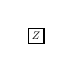
\begin{tikzpicture}
    \node[rectangle,draw,scale=0.4, fill=white] (r) at (0,0) {$Z$};
\end{tikzpicture}};
\node[scale=1.3] at (3.3,1/2){$0$};
\node[scale=2.10] at (3,0.8){% !TEX root = main.tex

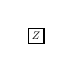
\begin{tikzpicture}
    \node[rectangle,draw,scale=0.4, fill=white] (r) at (0,0) {$Z$};
\end{tikzpicture}};
\node[scale=1.3] at (3.3,0.8){$1$};


\draw[line width=1.25] (0,0) -- (1,-0.5);
\draw[line width=1.25] (0,0) -- (1,-0.8);
\draw[line width=1.25] (0,0) -- (1,-1.1);
\draw[line width=1.25] (0,0) -- (1,-1.4);


\draw[line width=1.25] (3,-1/2) -- (0.985,-1/2);
\draw[line width=1.25] (3,-0.8) -- (0.985,-0.8);
\draw[line width=1.25] (3,-1.1) -- (0.985,-1.1);
\draw[line width=1.25] (3,-1.4) -- (0.985,-1.4);


\node[scale=2.10] at (3,-1.1){% !TEX root = main.tex

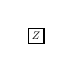
\begin{tikzpicture}
    \node[rectangle,draw,scale=0.4, fill=white] (r) at (0,0) {$Z$};
\end{tikzpicture}};
\node[scale=1.3] at (3.3,-1.1){$1$};
\node[scale=2.10] at (3,-1.4){% !TEX root = main.tex

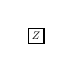
\begin{tikzpicture}
    \node[rectangle,draw,scale=0.4, fill=white] (r) at (0,0) {$Z$};
\end{tikzpicture}};
\node[scale=1.3] at (3.3,-1.4){$0$};

% \node[draw, scale=1.5, fill=white] at (3,-1/2){$P$};
% \node[draw, scale=1.5, fill=white] at (2,-1/2){$C$};
\node[draw, scale=3.1, fill=white] at (2.0,0.95){$C^{T}$};
\node[draw, scale=3.1, fill=white] at (2.0,-0.95){$C^{\dagger}$};
\node[anchor=east] at (5.5, 0) (node1){};
\node[anchor=east] at (5.5, -1.25) (node2){};

\draw [-latex,red, line width=0.55mm] (3.65,0.65) to [out=270-20,in=180-70] (3.65,-0.65);
\draw [-latex,blue, line width=0.55mm] (5.5,-0.65) to [in=290,out=70] (5.5,0.65);

\end{tikzpicture}
\end{subfigure}\hspace{35mm}
\begin{subfigure}[htp]{0.3\textwidth}
\begin{tikzpicture}[scale=1.5]

\draw[line width=1.25] (3,1/2) -- (1.25,1/2);
 \node[ellipse, draw, scale=5.7, draw=purple!90, fill=purple!45, fill opacity=0.8] at (3.7,0.95){};
\node[scale=2.6] at (3.75,0.95){$\ket{\psi_L}$};
\draw[line width=1.25] (3,0.8) -- (1.25,0.8);
\draw[line width=1.25] (3,1.1) -- (1.1,1.1);
 \node[ellipse, draw, scale=3.0, draw=purple!90, fill=purple!15, fill opacity=0.8] at (0.75,1.25){};
\node[scale=1.8] at (0.8,1.25){$\ket{\psi}$};
\draw[line width=1.25] (3,1.4) -- (1.1,1.4);
\node[scale=1.2] at (1,1/2){$\ket{0}$};
\node[scale=1.2] at (1,0.8){$\ket{0}$};

% \draw [->,red] (3.0,0.95) to [out=225,in=135] (3.0,-0.95);
\node[draw=none, scale=3.1] at (-0.4,0.95){$\simeq$};

\node[draw, scale=3.3, fill=white] at (2.0,0.95){$C$};
\end{tikzpicture}
\end{subfigure}